\documentclass[aspectratio=169,10pt]{beamer}
\usetheme{default}
\usecolortheme{seagull}
\setbeamertemplate{navigation symbols}{}
\setbeamertemplate{footline}[frame number]
\setbeamertemplate{itemize items}[circle]
\usepackage{booktabs,graphicx}
\newcommand{\blipMean}{73.1}
\newcommand{\blipMeanStd}{1.6}
\newcommand{\blipGreedy}{70.2}
\newcommand{\blipGreedyStd}{1.1}
\newcommand{\blipFactF}{80.4}
\newcommand{\blipFactFStd}{0.9}
\newcommand{\blipPresence}{91.7}
\newcommand{\blipIdentify}{69.3}
\newcommand{\blipExtent}{65.1}
\newcommand{\blipLocation}{66.4}
\newcommand{\zeroMean}{29.6}
\newcommand{\zeroMeanStd}{0.4}
\newcommand{\zeroGreedy}{16.4}
\newcommand{\zeroGreedyStd}{0.4}
\newcommand{\zeroFactF}{0.0}
\newcommand{\zeroFactFStd}{0.0}
\newcommand{\zeroPresence}{59.4}
\newcommand{\zeroIdentify}{13.4}
\newcommand{\zeroExtent}{41.1}
\newcommand{\zeroLocation}{4.3}
\newcommand{\voneMean}{67.7}
\newcommand{\voneMeanStd}{0.9}
\newcommand{\voneGreedy}{66.8}
\newcommand{\voneGreedyStd}{0.9}
\newcommand{\voneFactF}{58.3}
\newcommand{\voneFactFStd}{4.0}
\newcommand{\vonePresence}{89.9}
\newcommand{\voneIdentify}{59.3}
\newcommand{\voneExtent}{60.6}
\newcommand{\voneLocation}{60.9}
\newcommand{\vtwoMean}{68.1}
\newcommand{\vtwoMeanStd}{1.2}
\newcommand{\vtwoGreedy}{66.8}
\newcommand{\vtwoGreedyStd}{1.1}
\newcommand{\vtwoFactF}{76.8}
\newcommand{\vtwoFactFStd}{2.7}
\newcommand{\vtwoPresence}{90.5}
\newcommand{\vtwoIdentify}{60.4}
\newcommand{\vtwoExtent}{60.3}
\newcommand{\vtwoLocation}{61.0}
\newcommand{\blipRanked}{73.1}
\newcommand{\finalCycle}{5}
\newcommand{\finalPairs}{960k}
\newcommand{\finalVal}{71.5}
\newcommand{\blipPartial}{77.5}
\newcommand{\finalChange}{1.6}
\newcommand{\finalChangeLo}{0.8}
\newcommand{\finalChangeHi}{2.3}
\newcommand{\finalChangeFolds}{5}
\newcommand{\prevVal}{69.5}
\newcommand{\totalChange}{5.0}
\newcommand{\totalChangeLo}{3.7}
\newcommand{\totalChangeHi}{6.4}
\newcommand{\capChange}{3.6}
\newcommand{\capChangeLo}{1.2}
\newcommand{\capChangeHi}{6.0}
\newcommand{\capChangeFolds}{5}
\newcommand{\blipCorrMean}{74.6}
\newcommand{\blipCorrMeanStd}{1.4}
\newcommand{\corrChange}{1.5}
\newcommand{\corrChangeLo}{0.9}
\newcommand{\corrChangeHi}{2.0}
\newcommand{\corrChangeFolds}{5}
\newcommand{\corrIdentify}{75.1}
\newcommand{\corrNdTrue}{1,353}
\newcommand{\corrNdSaid}{481}
\newcommand{\corrValChange}{1.8}
\newcommand{\corrValLo}{1.2}
\newcommand{\corrValHi}{2.4}
\newcommand{\corrValFolds}{5}
\newcommand{\tfourHours}{64}
\newcommand{\proHours}{114}
\newcommand{\constMean}{42.4}
\newcommand{\constLocation}{57.3}
\newcommand{\constIdentify}{23.2}
\newcommand{\blipAccEighty}{83.9}
\newcommand{\blipAurc}{0.08}
\newcommand{\blipCreditAmb}{39.9}
\newcommand{\blipAccClear}{77.3}
\newcommand{\blipEce}{0.13}
\newcommand{\blipAccAll}{73.5}
\newcommand{\zeroAurc}{0.53}
\newcommand{\leakGap}{$-2.3$}
\newcommand{\leakLo}{$-6.5$}
\newcommand{\leakHi}{2.2}
\newcommand{\leakSeen}{72.3}
\newcommand{\leakUnseen}{74.6}
\newcommand{\ndviDiff}{0.1}
\newcommand{\ndviLo}{$-0.8$}
\newcommand{\ndviHi}{0.9}
\newcommand{\qwenRgbMean}{67.3}
\newcommand{\qwenRgbPooled}{70.3}
\newcommand{\qwenRgbPresence}{81.4}
\newcommand{\qwenRgbLocation}{62.1}
\newcommand{\qwenRgbFactF}{64.9}
\newcommand{\qwenRgbPrecision}{65.9}
\newcommand{\qwenRgbRecall}{64.0}
\newcommand{\qwenRgbDiff}{$-5.1$}
\newcommand{\qwenRgbWords}{9}
\newcommand{\referenceWords}{6}
\newcommand{\qwenNdviMean}{66.9}
\newcommand{\qwenNdviPooled}{70.4}
\newcommand{\qwenNdviPresence}{83.1}
\newcommand{\qwenNdviLocation}{61.5}
\newcommand{\qwenNdviFactF}{65.5}
\newcommand{\qwenNdviPrecision}{63.3}
\newcommand{\qwenNdviRecall}{67.7}
\newcommand{\qwenNdviDiff}{$-5.0$}
\newcommand{\qwenNdviWords}{9}
\newcommand{\blipFoldMean}{71.0}
\newcommand{\blipFoldPooled}{75.4}
\newcommand{\blipFoldPresence}{91.7}
\newcommand{\blipFoldLocation}{66.6}
\newcommand{\blipFoldFactF}{80.3}
\newcommand{\blipFoldPrecision}{78.2}
\newcommand{\blipFoldRecall}{82.5}
\newcommand{\blipFoldWords}{9}
\newcommand{\voneFoldMean}{67.7}
\newcommand{\voneFoldPooled}{72.6}
\newcommand{\voneFoldPresence}{90.5}
\newcommand{\voneFoldLocation}{61.9}
\newcommand{\voneFoldFactF}{61.3}
\newcommand{\voneFoldPrecision}{45.9}
\newcommand{\voneFoldRecall}{92.0}
\newcommand{\voneFoldDiff}{$-2.8$}
\newcommand{\voneFoldWords}{33}
\newcommand{\vtwoFoldMean}{67.6}
\newcommand{\vtwoFoldPooled}{72.5}
\newcommand{\vtwoFoldPresence}{90.6}
\newcommand{\vtwoFoldLocation}{63.3}
\newcommand{\vtwoFoldFactF}{77.3}
\newcommand{\vtwoFoldPrecision}{75.7}
\newcommand{\vtwoFoldRecall}{79.0}
\newcommand{\vtwoFoldDiff}{$-2.9$}
\newcommand{\vtwoFoldWords}{9}
\newcommand{\balancedMean}{66.5}
\newcommand{\balancedPooled}{71.7}
\newcommand{\balancedPresence}{91.0}
\newcommand{\balancedLocation}{56.0}
\newcommand{\balancedFactF}{77.3}
\newcommand{\balancedPrecision}{75.7}
\newcommand{\balancedRecall}{79.0}
\newcommand{\balancedDiff}{$-0.8$}
\newcommand{\balancedWords}{9}
\newcommand{\doraMean}{67.2}
\newcommand{\doraPooled}{72.2}
\newcommand{\doraPresence}{90.5}
\newcommand{\doraLocation}{62.9}
\newcommand{\doraFactF}{61.2}
\newcommand{\doraPrecision}{45.9}
\newcommand{\doraRecall}{92.0}
\newcommand{\doraDiff}{$-0.4$}
\newcommand{\doraWords}{33}
\newcommand{\blipParaphraseDrop}{8.3}
\newcommand{\blipJpegDrop}{24.8}
\newcommand{\blipBlurDrop}{15.6}
\newcommand{\blipNoiseDrop}{10.5}
\newcommand{\blipResDrop}{14.1}
\newcommand{\blipLightDrop}{2.8}
\newcommand{\blipFlipDrop}{0.3}
\newcommand{\blipRotDrop}{2.8}
\newcommand{\blipJpegAcc}{50.5}
\newcommand{\blipRobustClean}{75.3}
\newcommand{\blipPerturbed}{6.9}
\newcommand{\vtwoParaphraseDrop}{10.7}
\newcommand{\vtwoJpegDrop}{14.5}
\newcommand{\vtwoBlurDrop}{11.4}
\newcommand{\vtwoNoiseDrop}{4.7}
\newcommand{\vtwoResDrop}{9.9}
\newcommand{\vtwoLightDrop}{0.4}
\newcommand{\vtwoFlipDrop}{0.1}
\newcommand{\vtwoRotDrop}{0.6}
\newcommand{\vtwoJpegAcc}{57.3}
\newcommand{\vtwoRobustClean}{71.9}
\newcommand{\vtwoPerturbed}{3.9}
\newcommand{\voneParaphraseDrop}{11.3}
\newcommand{\voneJpegDrop}{14.4}
\newcommand{\voneBlurDrop}{9.5}
\newcommand{\voneNoiseDrop}{5.2}
\newcommand{\voneResDrop}{8.1}
\newcommand{\voneLightDrop}{0.6}
\newcommand{\voneFlipDrop}{$-0.0$}
\newcommand{\voneRotDrop}{1.0}
\newcommand{\voneJpegAcc}{57.3}
\newcommand{\voneRobustClean}{71.6}
\newcommand{\vonePerturbed}{3.9}
\newcommand{\servedRgbParaphraseDrop}{7.0}
\newcommand{\servedRgbFlipDrop}{1.2}
\newcommand{\servedRgbRotDrop}{1.9}
\newcommand{\servedNdviParaphraseDrop}{4.2}
\newcommand{\servedNdviFlipDrop}{$-1.0$}
\newcommand{\servedNdviRotDrop}{$-0.8$}
\newcommand{\blipMidJpeg}{12.3}
\newcommand{\blipMidBlur}{9.6}
\newcommand{\blipMidNoise}{4.9}
\newcommand{\blipMidRes}{7.0}
\newcommand{\blipMidLight}{0.6}
\newcommand{\servedRgbMidJpeg}{4.0}
\newcommand{\servedRgbMidBlur}{4.4}
\newcommand{\servedRgbMidNoise}{2.8}
\newcommand{\servedRgbMidRes}{2.1}
\newcommand{\servedRgbMidLight}{2.3}
\newcommand{\servedNdviMidJpeg}{2.3}
\newcommand{\servedNdviMidBlur}{3.4}
\newcommand{\servedNdviMidNoise}{$-0.4$}
\newcommand{\servedNdviMidRes}{2.0}
\newcommand{\servedNdviMidLight}{1.9}
\newcommand{\voneLocThroughout}{93.4}
\newcommand{\voneLocLocalised}{24.0}
\newcommand{\locNThroughout}{1,129}
\newcommand{\locNLocalised}{936}
\newcommand{\vtwoLocThroughout}{93.9}
\newcommand{\vtwoLocLocalised}{26.4}
\newcommand{\blipLocThroughout}{86.7}
\newcommand{\blipLocLocalised}{42.4}
\newcommand{\balLocThroughout}{77.1}
\newcommand{\balLocLocalised}{30.5}
\newcommand{\balLocDrop}{7.3}
\newcommand{\qwenZeroLenient}{14.2}
\newcommand{\pointZero}{39.3}
\newcommand{\pointLora}{56.3}
\newcommand{\pointChance}{33.1}
\newcommand{\energyZero}{34.5}
\newcommand{\energyLora}{43.4}

\title{Reading crop anomalies with LoRA-tuned vision--language models}
\subtitle{AI 512, Project 3: BLIP + LoRA on Agriculture-Vision, and a laptop-served VLM}
\date{\today}
\begin{document}
\frame{\titlepage}

\begin{frame}{The task}
\begin{columns}
\column{0.55\textwidth}
\begin{itemize}
\item Agriculture-Vision: aerial farmland tiles (512 px, about 10 cm/px, RGB + NIR) with expert pixel masks for nine anomalies.
\item Masks are precise but not readable. A farmer asks: \emph{is there standing water in this field, and where?}
\item The brief: fine-tune BLIP with LoRA to caption and answer such questions, and compare with zero-shot BLIP.
\item We add: a leakage test, selective answering, attention heatmaps, and a newer VLM served on a laptop CPU with an NDVI input.
\end{itemize}
\column{0.45\textwidth}
\small
\begin{tabular}{lr}
\toprule
Labelled tiles (train + val) & 75,278 \\
Fields & 1,741 \\
Views incl.\ quadrants & 348,124 \\
Most common class (drydown) & 29.7\% \\
Rarest class (storm damage) & 0.6\% \\
Tiles with 2+ anomalies & 6.3\% \\
\bottomrule
\end{tabular}
\end{columns}
\end{frame}

\begin{frame}{From masks to language}
One streaming pass turns every tile and quadrant into mask statistics; a generator turns those into text.
\medskip
\resizebox{\textwidth}{!}{\begin{tabular}{lll}
\toprule
Question type & Example & Answer vocabulary \\
\midrule
Presence & Is there weed cluster in this tile? & yes / no, balanced per view \\
Identify & What anomalies are visible? & class names, largest first, or \emph{none} \\
Extent & How much of the tile does the drydown cover? & small / moderate / large (cuts at 10\% and 35\%) \\
Location & Where is the standing water? & a 3$\times$3 grid cell, or \emph{throughout} \\
\bottomrule
\end{tabular}}

\medskip
Caption: ``Large drydown throughout the tile, with small weed cluster at the top left'', in one of five phrasings.
\medskip
\begin{itemize}
\item Ambiguous cases are flagged from the masks (near a cut point, under 1\% area, a near-tie between cells) and train on hedges: \emph{possibly}, \emph{small to moderate}, \emph{top left or centre}.
\item Clean examples come from anomaly-free quadrants (33,014 views); a balanced sampler up-weights rare classes.
\end{itemize}
\end{frame}

\begin{frame}{Method}
\begin{columns}
\column{0.5\textwidth}
\textbf{Graded: BLIP + LoRA}
\begin{itemize}
\item \texttt{blip-vqa-base} for questions, \texttt{blip-image-captioning-base} for captions, 384 px.
\item fp16 base, fp32 LoRA, cosine schedule, clipping, loss scaler.
\item One-knob-at-a-time sweep on fold 0's inner validation: rank, then learning rate, then target modules.
\item Final: rank 64, query/value adapters, LR capped at $2\!\times\!10^{-4}$, \finalPairs\ pairs per fold (length chosen on validation), best second-half check kept.
\end{itemize}
\column{0.5\textwidth}
\textbf{Served: a newer VLM for the laptop}
\begin{itemize}
\item Bake-off on 10k pairs: Qwen3.5-2B 0.560, LFM2.5-VL-1.6B 0.535, LFM2.5-VL-450M 0.469.
\item LoRA on the language model only, so adapters switch per request in llama.cpp.
\item Two variants: RGB, and RGB + an NDVI map as a second image.
\item Also: DoRA on one fold, and a model trained on the official split for the leakage test.
\end{itemize}
\end{columns}
\end{frame}

\begin{frame}{Evaluation: dynamic, field-grouped cross-validation}
\begin{itemize}
\item Tiles from one field are near-duplicates, so 5-fold \texttt{StratifiedGroupKFold} groups by field and stratifies on the rarest class. Folds are regenerated from a seed recorded per run; no split file is saved.
\item Each training fold holds out 10\% of its fields as inner validation for checkpoint choice. Test folds are never seen before final scoring.
\item Per fold about 2,000 test tiles, 11,000 questions and 2,200 captions. BLIP rows: 5 folds, mean $\pm$ std. Served rows: fold 0 with field-bootstrap 95\% intervals and paired differences.
\item Strict exact match after normalising. Headline readout: rank the type's fixed answer list by likelihood (chosen on validation); greedy generation reported too. Captions: fact precision/recall/F1 plus BLEU, ROUGE-L and CIDEr.
\item \textbf{The floor to clear:} the single best answer per question type, chosen with hindsight, scores \constMean\% on average.
\end{itemize}
\end{frame}

\begin{frame}{Zero-shot BLIP vs BLIP-LoRA}
\centering
\resizebox{\textwidth}{!}{\begin{tabular}{lccccccccc}
\toprule
Model & Presence & Identify & Extent & Location & Mean & BLEU-4 & ROUGE-L & CIDEr & Fact F1 \\
\midrule
Zero-shot BLIP & 59.4 $\pm$ 1.4 (59.5) & 13.4 $\pm$ 0.1 (6.1) & 41.1 $\pm$ 1.2 (0.0) & 4.3 $\pm$ 0.7 (0.0) & 29.6 $\pm$ 0.4 (16.4) & 0.0 $\pm$ 0.0 & 9.8 $\pm$ 0.4 & 0.01 & 0.0 $\pm$ 0.0 \\
Most common answer & 53.3 $\pm$ 0.0 & 23.2 $\pm$ 4.0 & 35.7 $\pm$ 1.9 & 57.3 $\pm$ 2.0 & 42.4 $\pm$ 1.2 & -- & -- & -- & -- \\
BLIP-LoRA v1 & 89.9 $\pm$ 0.4 (89.9) & 59.3 $\pm$ 1.8 (56.5) & 60.6 $\pm$ 2.3 (61.0) & 60.9 $\pm$ 2.3 (59.6) & 67.7 $\pm$ 0.9 (66.8) & 14.9 $\pm$ 0.9 & 40.7 $\pm$ 1.7 & 0.13 & 58.3 $\pm$ 4.0 \\
BLIP-LoRA v2 & 90.5 $\pm$ 0.9 (90.5) & 60.4 $\pm$ 1.0 (56.8) & 60.3 $\pm$ 3.4 (59.7) & 61.0 $\pm$ 2.1 (60.1) & 68.1 $\pm$ 1.2 (66.8) & 56.2 $\pm$ 4.9 & 73.5 $\pm$ 2.6 & 3.49 & 76.8 $\pm$ 2.7 \\
BLIP-LoRA & 91.3 $\pm$ 1.0 (91.3) & 73.8 $\pm$ 2.7 (59.3) & 64.8 $\pm$ 2.4 (63.6) & 66.3 $\pm$ 1.5 (64.7) & 74.0 $\pm$ 1.3 (69.7) & 60.2 $\pm$ 0.7 & 76.3 $\pm$ 0.3 & 3.86 & 80.4 $\pm$ 0.9 \\
\bottomrule
\end{tabular}
}
\begin{itemize}
\item Mean over question types: \zeroMean\% zero-shot, \constMean\% for the best constant answer, \blipMean\,$\pm$\,\blipMeanStd\% after LoRA under the ranked readout (greedy \blipGreedy\%), \textbf{\blipCorrMean\,$\pm$\,\blipCorrMeanStd\%} after the label-shift correction.
\item Presence \blipPresence\%, identify \blipIdentify\%, extent \blipExtent\%. Location \blipLocation\% against \constLocation\% for always saying \emph{throughout}: the smallest gain over its floor.
\item Caption fact F1 from 0 to \blipFactF\%; CIDEr stays near zero because every caption shares one template vocabulary.
\end{itemize}
\end{frame}

\begin{frame}{Every model on the same held-out items (fold 0)}
\centering
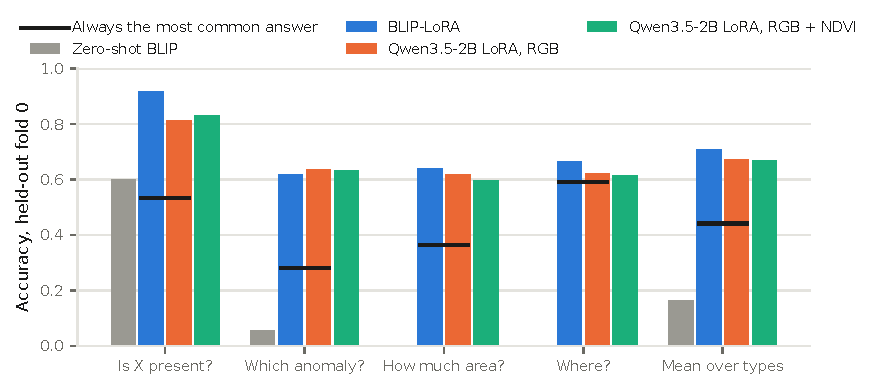
\includegraphics[width=0.92\textwidth]{figures/family_bars.pdf}
\end{frame}

\begin{frame}{Choosing rank, target modules and learning rate}
\centering
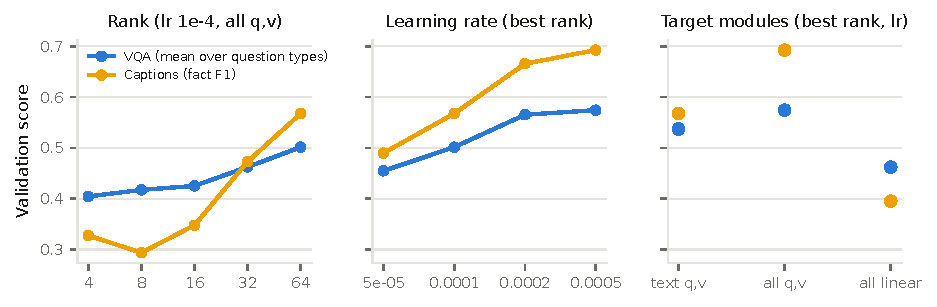
\includegraphics[width=0.95\textwidth]{figures/sweep.pdf}
\begin{itemize}
\item Rank is the clearest lever; learning rate the second. Text-only adapters are not enough: the image encoder must adapt to aerial imagery.
\item Both tasks prefer query/value adapters in every attention layer. (In v1, with captions that never ended, captions had preferred every linear layer.)
\end{itemize}
\end{frame}

\begin{frame}{A learning rate that only works for short runs}
\centering
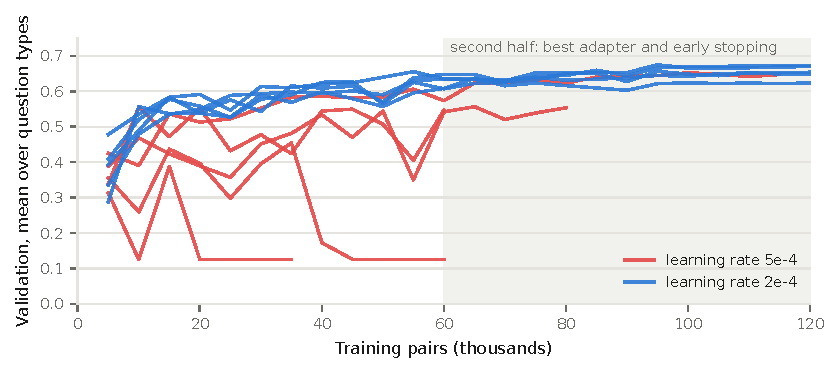
\includegraphics[width=0.9\textwidth]{figures/lr_curves.pdf}
\begin{itemize}
\item The 10k-pair sweep picked $5\!\times\!10^{-4}$. Held for 120k pairs it derailed 3 of 5 folds; two collapsed to one answer for everything.
\item Capped at $2\!\times\!10^{-4}$ (within a point in the sweep) every fold trains smoothly. Checkpoint choice and early stopping use second-half checks only.
\end{itemize}
\end{frame}

\begin{frame}{Hedging on ambiguous cases, and calibration}
\begin{columns}
\column{0.6\textwidth}
\resizebox{\textwidth}{!}{\begin{tabular}{lccccccc}
\toprule
Model & Hedge, amb. & Hedge, clear & Credit, amb. & Acc., clear & ECE & AURC & Acc. at 80\% cov. \\
\midrule
Zero-shot BLIP & 0.0 & 0.0 & 1.0 & 27.1 & 0.232 & 0.535 & 31.2 \\
BLIP-LoRA & 2.2 & 0.5 & 39.9 & 77.3 & 0.134 & 0.082 & 83.9 \\
Qwen3.5-2B LoRA, RGB & 0.0 & 0.0 & 37.3 & 72.1 & 0.118 & 0.145 & 75.1 \\
Qwen3.5-2B LoRA, RGB + NDVI & 0.0 & 0.0 & 36.7 & 72.2 & 0.109 & 0.145 & 75.2 \\
BLIP-DoRA v1 & 0.0 & 0.0 & 36.8 & 74.1 & 0.141 & 0.098 & 80.7 \\
\bottomrule
\end{tabular}
}
\medskip
\begin{itemize}
\item No model hedges in words: hedged targets are a tenth of the ambiguous families' pairs, so a committed answer is always likelier.
\item The signal is in the confidence: answering only the most confident 80\% lifts BLIP-LoRA to \blipAccEighty\% fully correct (AURC \blipAurc, against \zeroAurc\ zero-shot).
\item v2 adds a rule: hedge when the top two ranked answers are within a margin.
\end{itemize}
\column{0.4\textwidth}
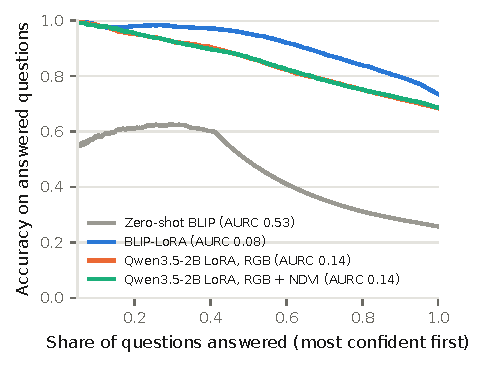
\includegraphics[width=\textwidth]{figures/risk_coverage.pdf}
\end{columns}
\end{frame}

\begin{frame}{Robustness: paraphrased questions and perturbed images}
\centering
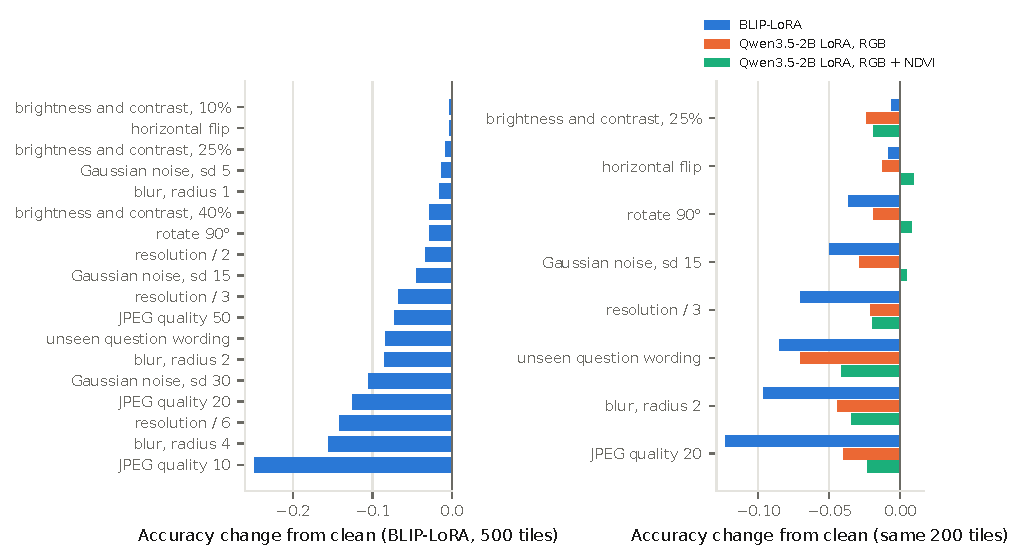
\includegraphics[width=0.95\textwidth,height=0.58\textheight,keepaspectratio]{figures/robustness.pdf}
\begin{itemize}
\item Lighting and flips cost at most \blipLightDrop; blur, noise and resolution degrade smoothly; heavy JPEG costs \blipJpegDrop.
\item Length made BLIP fragile: mean change over image perturbations $-$\vtwoPerturbed\ at 120k pairs, $-$\blipPerturbed\ at \finalPairs. Qwen loses less.
\item New wording: \blipParaphraseDrop\ for BLIP, \servedRgbParaphraseDrop\ and \servedNdviParaphraseDrop\ for Qwen RGB and NDVI.
\end{itemize}
\end{frame}

\begin{frame}{Augmentation removes most of the fragility}
\begin{itemize}
\item Cycle 4's fold-0 recipe retrained with half the training images damaged at random by the suite's own perturbation kinds.
\item Mean change over image perturbations: $-$\cFourPerturbed\ without, $-$\augFourPerturbed\ with. JPEG 10: $-$\cFourJpegDrop\ to $-$\augFourJpegDrop. Blur: $-$\cFourBlurDrop\ to $-$\augFourBlurDrop.
\item No clean cost on held-out fold 0: \augFourHeld\ points (95\% CI \augFourHeldLo\ to \augFourHeldHi). Validation \augFourVal\ against \augFourPlainVal.
\item At the final length (\finalPairs): $-$\cSixPerturbed\ without, $-$\augSixPerturbed\ with; held out \augSixHeld\ (95\% CI \augSixHeldLo\ to \augSixHeldHi). Five folds: validation \augFiveVal\% vs \finalVal\%, so the headline stays plain; held out \augFiveCorr\%, \augFiveChange\ over the headline (\augFiveChangeLo\ to \augFiveChangeHi). Reported as the deployable variant.
\item Same perturbation kinds as the test, so an upper bound for unfamiliar damage.
\end{itemize}
\end{frame}

\begin{frame}{Does the official split leak?}
\begin{columns}
\column{0.45\textwidth}
\resizebox{\textwidth}{!}{\emph{Pending: the official-split run is still training.}
}
\column{0.55\textwidth}
\begin{itemize}
\item 480 of the dataset's fields have flights in both official train and validation.
\item One BLIP-LoRA trained on official train: validation tiles from seen fields score \leakGap\ points \emph{lower} than unseen fields (95\% CI \leakLo\ to \leakHi).
\item No detectable inflation: the anomalies change between flights, so having seen a field does not give away its labels.
\item We still group folds by field: it costs nothing and keeps the comparison honest.
\end{itemize}
\end{columns}
\end{frame}

\begin{frame}{Where does the model look?}
\begin{itemize}
\item Gradient-weighted cross-attention for ``Is there \emph{X} in this tile?'' on 300 held-out tiles, scored against the mask (the pointing game).
\item Attention peak inside the anomaly: \pointZero\% zero-shot, \textbf{\pointLora\%} after LoRA, \pointChance\% by chance.
\item Attention energy on the mask: \energyZero\% to \energyLora\%.
\item Fine-tuning taught BLIP to look at the anomaly more often, though far from always.
\end{itemize}
\end{frame}

\begin{frame}{The served model, and does NDVI help?}
\centering
\resizebox{\textwidth}{!}{\begin{tabular}{lcccccccc}
\toprule
Model & Presence & Identify & Extent & Location & Mean & Pooled acc. [95\% CI] & $\Delta$ vs BLIP-LoRA & Fact F1 (P/R) \\
\midrule
Zero-shot BLIP & 60.1 & 5.4 & 0.0 & 0.0 & 16.4 & 25.8 [24.6, 26.9] & -49.4 [-52.3, -46.6] & 0.0 (0/0) \\
BLIP-LoRA v1 & 90.5 & 58.2 & 60.3 & 61.9 & 67.7 & 72.6 [70.2, 75.0] & -2.6 [-3.9, -1.5] & 61.3 (46/92) \\
BLIP-LoRA v2 & 90.6 & 57.2 & 59.4 & 63.3 & 67.6 & 72.5 [70.2, 75.1] & -2.6 [-3.8, -1.6] & 77.3 (76/79) \\
BLIP-LoRA & 92.1 & 59.9 & 64.5 & 66.0 & 70.6 & 75.2 [72.8, 77.7] & -- & 80.3 (78/82) \\
BLIP-DoRA v1 & 90.5 & 55.9 & 59.7 & 62.9 & 67.2 & 72.2 [69.9, 74.6] & -0.4 [-1.1, 0.3] & 61.2 (46/92) \\
BLIP-LoRA v2, balanced location draws & 91.0 & 57.2 & 61.8 & 56.0 & 66.5 & 71.7 [69.6, 74.1] & -0.8 [-1.6, -0.1] & 77.3 (76/79) \\
Qwen3.5-2B, zero-shot & 0.0 & 0.0 & 0.0 & 0.0 & 0.0 (14.2) & 0.0 [0.0, 0.0] & -75.2 [-77.7, -72.8] & 0.1 (100/0) \\
Qwen3.5-2B LoRA, RGB v1 & 72.4 & 58.8 & 57.9 & 62.1 & 62.8 & 64.9 [62.7, 67.2] & -10.3 [-11.8, -8.8] & 56.4 (58/55) \\
Qwen3.5-2B LoRA, RGB & 81.4 & 63.6 & 61.9 & 62.1 & 67.3 & 70.3 [68.2, 72.7] & -4.9 [-6.3, -3.4] & 64.9 (66/64) \\
Qwen3.5-2B LoRA, RGB + NDVI v1 & 76.9 & 59.1 & 58.7 & 62.9 & 64.4 & 67.1 [65.1, 69.3] & -8.1 [-9.6, -6.6] & 60.6 (60/61) \\
Qwen3.5-2B LoRA, RGB + NDVI & 83.1 & 63.4 & 59.6 & 61.5 & 66.9 & 70.4 [68.2, 72.7] & -4.8 [-6.5, -3.2] & 65.5 (63/68) \\
\midrule
NDVI minus RGB & \multicolumn{6}{c}{} & 0.1 [-0.8, 0.9] & \\
\bottomrule
\end{tabular}
}
\begin{itemize}
\item Qwen3.5-2B after 60k pairs: \qwenRgbMean\% (RGB), \qwenNdviMean\% (RGB + NDVI), greedy like BLIP's row here. Most of its gap is presence; captions \qwenNdviPrecision\% precise against BLIP's \blipFoldPrecision\%.
\item NDVI: \ndviDiff\ points overall (95\% CI \ndviLo\ to \ndviHi). Presence F1 rises for drydown (+7.0) and nutrient deficiency (+6.1), the anomalies that change near-infrared reflectance, and is flat for most others.
\item DoRA matches LoRA (\doraDiff\ points) at 29\% more training time.
\end{itemize}
\end{frame}

\begin{frame}{On a laptop CPU}
\begin{columns}
\column{0.55\textwidth}
\begin{itemize}
\item FastAPI backend, llama.cpp serving the Q4 Qwen3.5-2B with both LoRA adapters loaded; the adapter is chosen per request.
\item Zero-shot BLIP alongside, for a before/after view.
\item A map with a drag-to-select field box, one chat panel: caption, findings with confidences, answers streamed as generated.
\item Satellite context (Sentinel-2 NDVI, HLS season series, weather) is shown, never model input.
\end{itemize}
\column{0.45\textwidth}
\small
\begin{tabular}{lr}
\toprule
Read a tile, RGB adapter & about 4 s \\
Read a tile, NDVI adapter & about 7 s \\
Switch adapters & free \\
Model + adapters in RAM & about 3 GB \\
\bottomrule
\end{tabular}
\end{columns}
\end{frame}

\begin{frame}{Second cycle: four findings from the first}
\begin{itemize}
\item \textbf{Captions never ended.} \texttt{blip-image-captioning-base} gives a full stop a loss near 13 nats and every target ended in one, so captions ran to \voneFoldWords\ words against \referenceWords\ in the truth (precision \voneFoldPrecision\%). Fix: targets end on their last word. Fold-0 fact F1 \voneFoldFactF\% $\to$ \blipFoldFactF\% (validation 0.631 $\to$ 0.839).
\item \textbf{Early stopping fired on noise.} Patience 3 on a 300-tile validation set: every VQA fold stopped at 80--115k pairs while its last six checks sat within 0.6--3.4 points. Fix: the full 120k pairs, best second-half check.
\item \textbf{Location: do not rebalance the draws.} 55\% of truths are \emph{throughout}; the first cycle scored \voneLocThroughout\% on those and \voneLocLocalised\% on localised items. Drawing cells 65\% of the time lifted localised items to \balLocLocalised\% but cost \balLocDrop\ points on the natural mix. The final sampler keeps the data's own draws; both adapters are kept.
\item \textbf{Five phrasings looked too few.} Twelve now, no synonym shared with the held-out set: paraphrase drop \voneParaphraseDrop\ $\to$ \vtwoParaphraseDrop\ points, barely less; longer training took it to \blipParaphraseDrop.
\item \textbf{Qwen:} 30k more pairs on the corrected targets, warm-started from cycle 1.
\end{itemize}
\end{frame}

\begin{frame}{What raised the ceiling? A study on validation}
\begin{itemize}
\item One change at a time from the v2 recipe on fold 0, 30k pairs, 1,000 inner-validation tiles. Three seeds of the unchanged recipe span 56.5--58.2: a single run carries about a point of noise.
\item At 30k, capacity helps a little: rank 256 +1.3 (two seeds), every linear layer +1.7 at $3.4\times$ the parameters. At 120k neither holds (+0.6 and +0.8, intervals across zero).
\item Dropout, $\alpha$, LayerNorms, 512 px, a NIR--red--green image: within noise. BLIP-large captions: no better at $4\times$ the compute; no BLIP-large VQA checkpoint exists.
\item \textbf{Length} is far outside the noise: +2.6 at 60k, +4.4 at 120k, +5.5 at 240k, +6.9 at 480k.
\item Readout: ranking the fixed answer list beats greedy by 1.1 (0.4 to 1.8); beam search $-0.2$; flip/rotation averaging $+0.0$; two-seed averaging +0.8 against +1.9 for the same compute spent on length.
\end{itemize}
\end{frame}

\begin{frame}{Length, chosen on validation, confirmed held out}
\begin{columns}
\column{0.58\textwidth}
\resizebox{\textwidth}{!}{\begin{tabular}{crcccccc}
\toprule
Cycle & Pairs & Validation & Held out, ranked & Change [95\% CI], folds up & Held out, greedy & Partial credit & Perturbed images \\
\midrule
2 & 120k & -- & 68.1 $\pm$ 1.2 & -- & 66.8 $\pm$ 1.1 & 72.7 $\pm$ 1.2 & $-3.9$ \\
3 & 240k & 68.2 & 70.2 $\pm$ 1.2 & +2.2 [+1.1, +3.2], 5/5 & 68.8 $\pm$ 1.4 & 74.7 $\pm$ 1.0 & $-4.9$ \\
4 & 480k & 69.5 & 71.5 $\pm$ 1.6 & +1.3 [+0.7, +1.9], 5/5 & 69.6 $\pm$ 1.5 & 76.0 $\pm$ 1.5 & $-5.0$ \\
5 & 960k & 71.5 & 73.1 $\pm$ 1.6 & +1.6 [+0.8, +2.3], 5/5 & 70.2 $\pm$ 1.1 & 77.5 $\pm$ 1.5 & $-6.9$ \\
\bottomrule
\end{tabular}
}
\medskip
\begin{itemize}\small
\item Rule fixed before any of these held-out scores were read: the cycle with the best five-fold validation wins. Held-out folds never choose.
\item Cycle \finalCycle\ (\finalPairs): \textbf{\blipMean\%} held out, +\finalChange\ over the cycle before (\finalChangeLo\ to \finalChangeHi, \finalChangeFolds/5 folds), +\totalChange\ over cycle 2.
\item Captions at 480k: fact F1 \vtwoFactF\% $\to$ \blipFactF\%.
\item Training draws are balanced; the test is not. Correcting the ranking for that shift, fitted on validation (+\corrValChange, \corrValFolds/5 folds): \textbf{\blipCorrMean\%} held out, +\corrChange\ (\corrChangeLo\ to \corrChangeHi, \corrChangeFolds/5), all on identify.
\item Corrected, cycle \finalCycle\ adds only \corrStep\ over the cycle before (\corrStepLo\ to \corrStepHi, \corrStepFolds/5): returns from length are shrinking. Cycle 7 (fold 0): validation \sevenVal\% vs \sixValZero\%, held out \sevenHeldZero\% vs \sixHeldZero\%.
\end{itemize}
\column{0.42\textwidth}
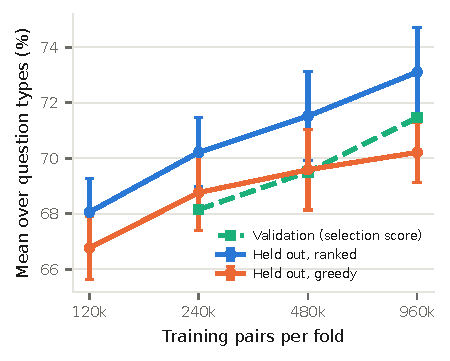
\includegraphics[width=\textwidth]{figures/length_curve.pdf}
\end{columns}
\end{frame}

\begin{frame}{Underfit, not memorised}
\begin{itemize}
\item Fold 0's adapters scored on 2,000 of their own training tiles, drawn by the held-out rules.
\item Cycle 2: \fitTwoTrain\% seen against \fitTwoHeld\% held out. Cycle \finalCycle: \fitTrain\% against \fitHeld\%. The gap widens from \fitTwoGap\ to \fitGap\ points.
\item On seen tiles: presence \fitPresence\%, extent \fitExtent\%, location \fitLocation\%. Clear pairs \fitClear\%, ambiguous credit \fitAmbig\%.
\item 98\% held out would first need extent and location fitted on fields the model has already seen.
\end{itemize}
\end{frame}

\begin{frame}{Limitations and conclusions}
\begin{itemize}
\item BLIP reads RGB only while the annotators also saw near infrared; extent is the only severity signal; captions come from templates; served rows use one fold; NDVI from these cameras is relative.
\item Masks can be turned into language that a small VLM learns to read: LoRA lifts BLIP from below a constant-answer floor to \blipCorrMean\% of questions right on unseen fields, with confidence that supports abstaining.
\item After the fixes, length beat capacity: rank, target modules, input size and BLIP-large stayed inside seed noise, while four doublings of training pairs added \totalChange\ points held out.
\item A learning rate that wins a short sweep can fail a long run; the official split's shared fields turned out harmless; a near-infrared view helps exactly the anomalies it should.
\item Code: \url{github.com/rit3sh-x/farmland-vlm}. Every table and figure rebuilds from the run records.
\end{itemize}
\end{frame}
\end{document}
